\section{Resistenz gegen Overfitting}
% \subsection{Neueste Forschungsergebnisse}
% \subsection{Zukünftige Potenziale von Boosting-Algorithmen}
Overfitting beschreibt das Phänomen, dass durch viele Trainingsiterationen das Modell so gut an die Trainingsdaten angepasst ist, dass es nicht mehr genug generalisiert und mit zunehmenden Iterationen sich der Testfehler erhöht.

\begin{figure}[H]
    \centering
    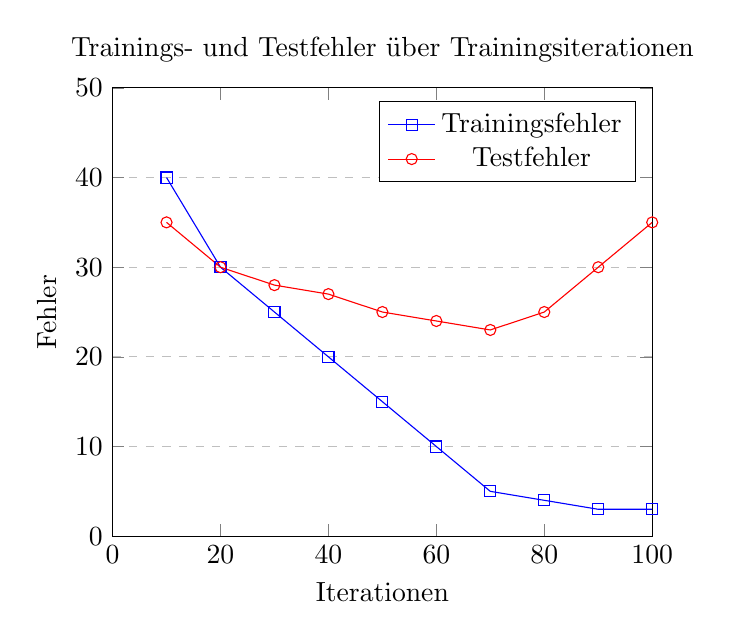
\begin{tikzpicture}
    \begin{axis}[
        title={Trainings- und Testfehler über Trainingsiterationen},
        xlabel={Iterationen},
        ylabel={Fehler},
        xmin=0, xmax=100,
        ymin=0, ymax=50,
        legend pos=north east,
        ymajorgrids=true,
        grid style=dashed,
    ]
    
    \addplot[
        color=blue,
        mark=square,
        ]
        coordinates {
        (10,40)(20,30)(30,25)(40,20)(50,15)(60,10)(70,5)(80,4)(90,3)(100,3)
        };
        \addlegendentry{Trainingsfehler}
    
    \addplot[
        color=red,
        mark=o,
        ]
        coordinates {
        (10,35)(20,30)(30,28)(40,27)(50,25)(60,24)(70,23)(80,25)(90,30)(100,35)
        };
        \addlegendentry{Testfehler}
    
    \end{axis}
    \end{tikzpicture}
    \caption[Hypothetische Darstellung von Overfitting]{Hypothetische Darstellung von Overfitting: Während der Trainingsfehler mit zunehmenden Iterationen abnimmt, beginnt der Testfehler nach einem gewissen Punkt wieder zu steigen.}
\end{figure}


\subsection{AdaBoost und die Herausforderung des Overfittings}
In \textcite[Kapitel 1.2.3]{SchapireFreund2012} wird das Phänomen des Overfitting für AdaBoost gezeigt. Trotz dieses theoretischen Hintergrunds war es mir in meinen praktischen Experimenten mit der SKLearn-Bibliothek in Python nicht möglich, Overfitting bei AdaBoost zu reproduzieren. Meine unzähligen Versuche mit unterschiedlichsten Anpassungen führten nicht zu den erwarteten Ergebnissen. Dies führt zu der Frage, warum AdaBoost in meinen Experimenten anscheinend resistent gegen Overfitting war. Der folgende Teil ist meine Theorie zu diesem Phänomen und entspricht nicht zwangsweise dem tatsächlichen Grund. Dieses eigene Beispiel sowie die Abbildungen wurden mithilfe von SKLearn in Python erstellt. Die Implementierung ist auf \textbf{\href{https://github.com/CodeLtDave/Boosting-Algorithms-ML-Seminararbeit/blob/main/python-env/ToleranceOverfittingAdaBoost.ipynb}{meinem GitHub repo}} zu finden.

\subsection{Wahl des Datensatzes}

Ich habe mich für einen der vielen Varianten an Datensätzen entschieden um Overfitting möglichst zu provozieren:

\begin{lstlisting}
    X, y = make_classification(n_samples=200, n_features=2, n_informative=2, n_redundant=0, n_clusters_per_class=1, flip_y=0.4, random_state=1)
\end{lstlisting}    
Ein relevanter Punkt ist die Menge der Datenpunkte `n\_samples'. Ist dieser zu hoch 
gewählt, ist es für das Modell zu leicht zu generalisieren. Mit den hier gewählten 200 Datenpunkten neigte AdaBoost schon deutlich eher zum Overfitting als beispielsweise mit 10,000.
\newline
Ein zusätzlicher Teil ist die Auswahl Attribute. In dem Datensatz werden zwei Attribute `n\_features' verwendet. Normalerweise würde dies gut klassifizierbare Daten erstellen. Allerdings werden 40\% der Datenwerte hier mittels `y\_flip' umgekehrt. Dies führt zu einem Datensatz, der keine eindeutige Klassifizierung erlaubt und viel Rauschen beeinhaltet.

\subsection{Ergebnisanalyse}
\begin{figure}[h]
    \centering
    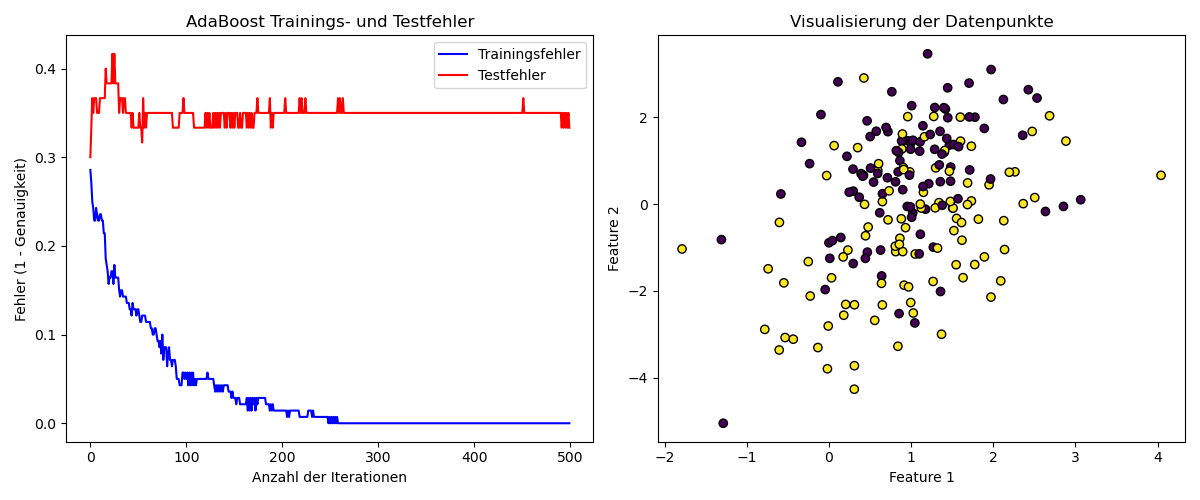
\includegraphics[width=0.8\textwidth]{Images/AdaBoost_Error_and_Data.png}
    \caption{Trainings- und Testfehler des AdaBoost-Modells über die Iterationen.}
    \label{fig:adaboost_error_plot}
\end{figure}
In \autoref{fig:adaboost_error_plot} sind die Ergebnisse des AdaBoost-Algorithmus dargestellt. Interessanterweise zeigt sich, dass obwohl der Trainingsfehler stetig abnimmt, dass der Testfehler nicht in dem Maße ansteigt, wie man es bei klassischem Overfitting erwarten würde. Stattdessen bleibt er sehr konstant.

\subsection{Philosophisches Prinzip: Occams Racor}
Occams Racor, oder auf deutsch Occams Rasiermesser ist ein philosophisches Prinzip, welches besagt, dass wenn es zwei Hypothesen zu einer Theorie gibt, dass die simplere vorzuziehen ist. Im Kontext des maschinellen Lernens, bedeutet dies, dass einfacherer Modelle den komplexeren vorzuziehen sind, da es anzunehmen ist, dass sie besser generalisieren. Dieses Prinzip suggeriert, dass bei der Klassifizierung unseres speziellen Datensatzes ein einfacheres Modell mit 250 Iterationen effektiver ist als das Endmodell mit 500 Iterationen, da es weniger anfällig für das `Auswendiglernen' spezifischer Muster der Trainingsdaten und somit für Overfitting ist.

\subsection{Erklärungsansatz: Margins Theorie}
Eine Grundeigenschaft von AdaBoost ist, dass die Gewichtung \(\alpha\) jedes Lerners zum Gesamtmodell immer vom Beitrag zum Gesamtmodell abhängt. Für die Frage, warum sich der Testfehler nicht verschlechtert, könnte dies ab der 250. Iteration eine Antwort sein, da ab diesem Punkt der Trainingsfehler nahe 0 is und sich das Modell nicht mehr verbessert. Dies kann aber offensichtlich nicht der Grund sein, da das Phänomen des konstanten Testfehlers auch bereits vor der 250. Iteration auftritt.
\newline
Die Margins Theorie im Kontext von AdaBoost bietet eine mögliche Erklärung. Diese Theorie konzentriert sich auf den Abstand der Datenpunkte zur Entscheidungsgrenze des Klassifizierers, also den Margin. Die Entscheidungsgrenzen sind in \autoref{fig:adaboost_decision_boundries} dargestellt. Ein größerer Margin impliziert eine höhere Zuversicht in die Klassifizierung. Gegensätzlich dazu ist ein geringer Margin, also eine kleine Distanz zur Entscheidungsgrenze ein Zeichen für eine geringe Zuversicht in die Klassifizierung.
\begin{figure}[h]
    \centering
    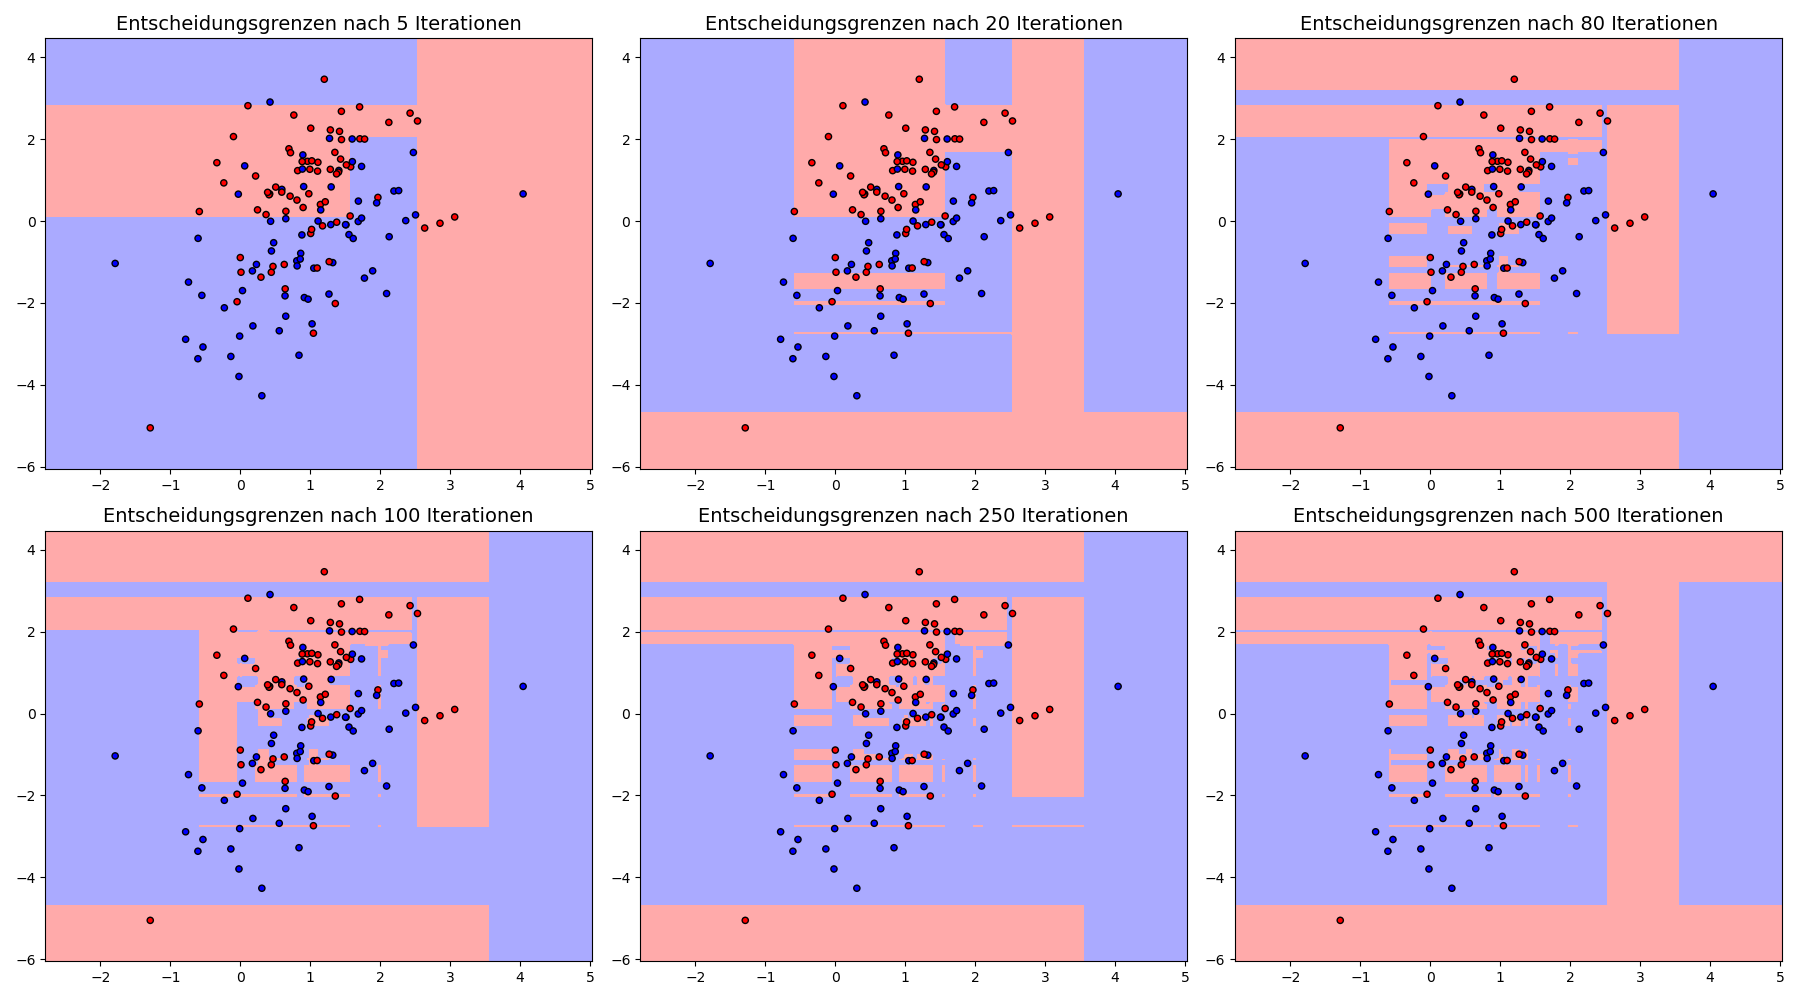
\includegraphics[width=\textwidth]{Images/AdaBoost_Multiple_Decision_Boundaries.png}
    \caption{Entscheidungsgrenzen des Modells}
    \label{fig:adaboost_decision_boundries}
\end{figure}
\paragraph{Einfluss auf die Entscheidungsgrenzen}
In \autoref{fig:adaboost_decision_boundries} sind die Entscheidungsgrenzen des AdaBoost-Modells dargestellt. Es ist erkennbar, dass die Grenzen mit zunehmenden Iterationen präziser werden. Dies bedeutet jedoch nicht automatisch eine steigende Komplexität des Modells. Insbesondere bis zur 250. Iteration konzentriert sich AdaBoost darauf, die Margins zu vergrößern, was bedeutet, dass es die Entscheidungsgrenze so anpasst, dass die Klassifizierungen sicherer werden. Also sich möglichst nicht direkt an den Datenpunkten liegen, was wie wir wissen, eine höhere Zuversicht auf die Richtigkeit der Vorhersage widerspiegelt.

\paragraph{Vermeidung von Overfitting}
Die Vergrößerung der Margins trägt also dazu bei, dass das Modell nicht übermäßig an die Trainingsdaten anzupassen. Durch die Fokussierung auf schwierigere Fälle und die Erhöhung der Margins für diese Datenpunkte kann AdaBoost Overfitting vermeiden. 

\paragraph{Zusammenfassung}
Die Margins Theorie ist also eine plausible Erklärung dafür, wie AdaBoost die Balance zwischen hoher Trainingsgenauigkeit und der Vermeidung von Overfitting hält. Die Fähigkeit des Modells, die Margins effektiv zu vergrößern und dabei die Entscheidungsgrenzen anzupassen, ohne dabei die Generalsierung zu verringern. \textbf{Diese Zuverlässigkeit gegen Overfitting macht Boosting Algorithmen so essentiell und populär.}

% \subsection{Exponentieller Abstieg des Trainingfehlers}
% !!! VERWEISEN